%algoritimi de parsere ( ierarhia + informatii despre ei + gramaticile particulare (ex gramatica de expresii))
\chapter{Algoritmi de parsare}
\label{Chapter3}
\lhead{Capitolul 3. \emph{Algoritmi de parsare}}

\section{Problema pars\v arii}
Problema recunoa\c sterii \^ in gramatici independente de context este urm\v atoarea: Dat\v a o
gramatic\v a G = (V, T, S, P) \c si un cuv\^ ant w$\in T^{*}$, care este r\v aspunsul la \^ intrebarea w$\in$L(G)? Se
\c stie c\v a problema este decidabil\v a; mai mult, exist\v a algoritmi care \^ in timp O($|w|^{3}$) dau r\v aspunsul la \^ intrebare (Cooke-Younger-Kasami, Earley, vezi [Gri86]).
Problema pars\v arii(analizei sintactice) este problema recunoa\c sterii la care se adaug\v a: dac\v a r\v aspunsul la \^ intrebarea w$\in$L(G) este afirmativ, se cere arborele sintactic (o reprezentare
a sa) pentru w. 

%Fie G = (V, T, S, P) o gramatică
%şi w∈L(G). Să notăm prin $\overset{p}%{\underset{st}{\Rightarrow}}$
% ($\overset{q}{ \underset {dr} {\Rightarrow}}$) relaţia de derivare extrem stângă(dreaptă) în care, pentru rescriere s-a aplicat producţia p∈P (q∈P). 
\section{Analiza sintactic\v a descendent\v a}
Analiza sintactic\v a descendent\v a
(parsarea descendent\v a) poate fi considerat\v a ca o tentativ\v a
de determinare a unei deriv\v ari extrem st\^ angi pentru un cuv\^ ant de intrare. \^ In termenii arborilor sintactici, acest lucru \^ inseamn\v a tentativa de construire a unui arbore sintactic pentru cuv\^ antul de intrare, pornind de la r\v ad\v acin\v a \c si construind nodurile \^ in manier\v a descendent\v a, \^ in preordine (construirea r\v adacinii, a subarborelui st\^ ang apoi a celui drept).Pentru realizarea acestui fapt avem nevoie de urm\v atoarea structur\v a
(figura 3.1):
\begin{itemize}
\item
{
	o band\v a de intrare \^ in care se introduce cuv\^ antul de analizat, care se parcurge de la st\^ anga la dreapta, simbol cu simbol; 
}
\item
{
	o memorie de tip stiv\v a(pushdown) \^ in care se ob\c tin formele propozi\c tionale st\^ angi(\^ incep\^ and cu S). Prefixul formei propozi\c tionale format din terminali se compar\v a cu simbolurile curente din banda de intrare ob\c tin\^andu-se astfel criteriul de \^ inaintare \^ in aceast\v a band\v a; 
}
\item
{
	o band\v a de ie\c sire \^ in care se \^ inregistreaz\v a pe r\^ and produc\c tiile care s-au aplicat \^ in derivarea extrem st\^ ang\v a care se construie\c ste. 
}

\end{itemize}

\begin{figure}[htbp]
\centering
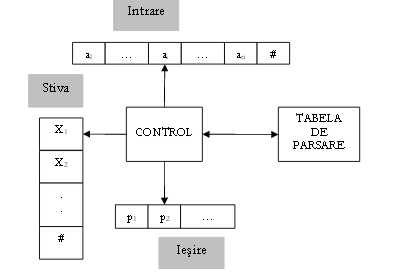
\includegraphics[scale=1]{parser_descendent.png}
	\rule{35em}{0.5pt}
\caption{Reprezentarea unui parser descendent}
	\label{fig:ParserDescendent}
\end{figure}

%\begin{figure}[htbp]
%	\centering
		%
\includegraphics{./Figures/Electron.pdf}
%		\rule{35em}{0.5pt}
%	\caption[An Electron]{An electron %(artist's impression).}
%	\label{fig:Electron}
%\end{figure}

Criteriul de oprire cu succes este acela \^ in care s-a parcurs \^ intreaga band\v a de intrare, iar memoria pushdown s-a golit. \^ In acest caz \^ in banda de ie\c sire s-a ob\c tinut parsarea st\^ ang\v a a cuv\^ antului respectiv. Iat\v a
un exemplu de cum func\c tioneaz\v a
acest mecanism (consider\v am
gramatica din exemplul precedent
\c si cuv\^ antul w = id+id*id). Vom considera caracterul \# pentru marcarea sf\^ ar\c sitului benzii de intrare (marca de sf\^ ar\c sit a cuv\^ antului) precum \c si pentru a marca baza stivei. 

\subsection{Gramaticile LL(1)}
Pentru ca un parser SLL(k) s\v a
poată fi implementat, trebuie s\v a
indic\v am o procedur\v a
pentru calculul mul\c timilor $FIRST_{k}$ \c si $FOLLOW_{k}$. Pentru c\v a \^ in practic\v a
se folose\c ste destul de rar (dac\v a nu chiar deloc) cazul k $\geq$ 2, vom restr\^ ange discu\c tia pentru cazul k=1. Vom nota \^ in acest caz $FIRST_{1}$ şi $FOLLOW_{1}$
prin FIRST respectiv FOLLOW.
A\c sadar, dac\v a
$\alpha\in \Sigma^{+}$, A$\in$V : \\
FIRST($\alpha$) = $\{a| a\in$T,$\alpha \overset{*}{\underset{st}{\Rightarrow}} au \}\cup$
if $(\alpha\overset{*}{\underset{st}{\Rightarrow}} \varepsilon)$ then ${\varepsilon}$ else $\emptyset$. \\
FOLLOW(A) = $\{a|a\in T \cup{\varepsilon}, S\overset{*}{\underset{st}{\Rightarrow}}uA\gamma$, $a\in FIRST (\gamma) \}$
Mai \^ int\^ ai s\v a ar\v at\v am c\v a gramaticile SLL(1) coincid cu gramaticile LL(1).  
\begin{theorem}
 O gramatic\v a G = (V, T, S, P) este gramatic\v a LL(1) dac\v a \c si numai dac\v a pentru orice $A \in V$ \c si pentru orice produc\c tii $A\rightarrow \beta_{1}|\beta_{2}$
are loc:
 \begin{flushleft}
 FIRST ($\beta_{1}$FOLLOW (A))$\cap$ 	FIRST($\beta_{2}$FOLLOW(A))=$\emptyset$
 \end{flushleft}

\end{theorem}
\subsection{Determinarea mul\c timilor FIRST \c si FOLLOW }
Vom indica \^ in acest paragraf modalitatea de determinare a mul\c timilor FIRST \c si FOLLOW pentru o gramatic\v a G.Un algoritm pentru determinarea mul\c timilor FIRST(X) este descris mai jos.\\
\textbf{Intrare:} Gramatica G=(V,T,S,P) redus\v a;\\
\textbf{Iesire:} FIRST(X),X$\in \Sigma$.\\
\textbf{Metoda:}Mul\c timile FIRST sunt completate prin inspectarea regulilor gramaticii\\
\begin{alltt}
1.for (X \(\in \Sigma\))
2.	if (X\( \in\)T) FIRST(X) = \({ X }\) else FIRST(X)=\(\emptyset\);
3.for (A \(\rightarrow \alpha \beta \in P\))
4.	FIRST (A) = FIRST(A) \(\cup\) \{ a \};
5.FLAG = true;
6.while(FLAG) \{ // FLAG marcheaza schimbarile in FIRST
7.	FLAG = false;
8.	for( \(A \rightarrow X1 X2 \ldots Xn \in P \)) \{
9.		i = 1;
10.     if((FIRST(X1)\(\nsubseteq\)FIRST(A)) \{
11.     	FIRST(A) = FIRST(A)\(\cup\)(FIRST(\(X1\));
12.			FLAG = true;
		\}//endif
13.		while(i<n && Xi\(\overset{+}{\underset{st}{\Rightarrow}}\)\(\varepsilon \) )
14.			if((FIRST(Xi+1)\( \nsubseteq \)FIRST(A)) \{
15.				FIRST(A) = FIRST(A)\(\cup\)FIRST(Xi+1);
16.				FLAG = true; i++;
			\}//endif
		\}//endwhile
	\}//endfor
\}//endwhile
17.for (A\(\in \)V)
18.if(A\( \overset{+}{\underset{st}{\Rightarrow}}\)\(\varepsilon \)) FIRST(A) = FIRST(A)\(\cup\)\{ \(\varepsilon \)\} ; 

\end{alltt}

Algoritmul pentru descrierea mul\c timilor FOLLOW:\\
\textbf{Intrare:} Gramatica G=(V,T,S,P) redus\v a;Procedura FIRST($\alpha$),$\alpha \in \Sigma^{+}$. \\
\textbf{Iesire:} Mul\c timile FOLLOW(A),A $\in$ V\\
\textbf{Metoda:} \\

\begin{alltt}
1.for (A\(\in \Sigma\)) FOLLOW(A) =\(\emptyset \);
2.FOLLOW(S)= \{\(\varepsilon \)\} ;
3.for (A\(\rightarrow \)X1X2...Xn) \{
4.	i = 1;
5.	while (i<n) \{
6.		while (Xi\(\notin \)V) ++i;
7.		if (i<n) \{// Xi este neterminal
8.			FOLLOW(Xi) = FOLLOW(Xi)\(\cup\)(FIRST(Xi+1Xi+2...Xn)-\{\(\varepsilon\)\});
9.			++i;
		\}//endif
	\}//endwhile
\}//endfor
10.FLAG = true;
11.while (FLAG) \{ // FLAG semnaleaza schimbarile in FOLLOW
12.	FLAG = false;
13.	for (A\( \rightarrow\)X1X2...Xn) \{
14.		i = n;
15.		while (i\(\geq\)1 && Xi \(\in\)V)\{
16.			if (FOLLOW (A)\(\nsubseteq \)FOLLOW(Xi) )\{
17.FOLLOW(Xi) = FOLLOW(Xi)\(\cup \)FOLLOW (A);
18.FLAG = true;
\}//endif
19.if(Xi\(\overset{+}{\underset{st}{\Rightarrow}}\)\(\varepsilon\))--i;// la Xi-1 daca Xi se sterge
20. else continue; // la urmatoarea productie
		\}//endwhile
	\}//endfor
\}//endwhile 
\end{alltt}

\subsection{Tabela de analiz\v a sintactic\v a LL(1)}
Pentru a implementa un analizor
sintactic pentru gramatici LL(1), s\v a consider\v am o tabel\v a de analiz\v a, sau
tabel\v a de parsare LL(1):\\
\begin{flushleft}
  M : V$\times$(T $\cup$ \{ \# \})
   $\rightarrow$ \{($\beta$,p)|p =$A \rightarrow \beta \in P$ \}   $\cup$ \{eroare\} 
  \end{flushleft}  
construit\v a dup\v a algoritmul urm\v ator: \\
\textbf{Intrare}  Gramatica G = (V, T, S,P); 
Mul\c timile FIRST($\beta$), FOLLOW(A), A$\rightarrow \beta \in $P. \\
\textbf{Iesire} Tabela de parsare M.\\
\textbf{Metoda} Se parcurg regulile gramaticii \c si se pun \^in tabel\v a\\
\begin{alltt}
1.for(A\(\in\)V) 
2.	for(a \(\in\) T \(\cup\) \{ # \})
3. 	   M(A,a)=\( \emptyset \);
4.for(p=A\( \rightarrow\beta \in \)P \{
5. for(a \( \in \) FIRST(\( \beta \))- \(\{ \varepsilon \} \))
6.		M(A,a)=M(A,a)\( \cup \)\{(\( \beta \),p )\};
7.	if(\(\varepsilon \in\) FIRST(\( \beta \))\{
8. 		for(b \( \in \) FOLLOW(A)) \{
9.			if(b == \(\varepsilon \)) M(A,\#)=M(A,\#) \( \cup \) \{(\(\beta\),p)\};
10.			else M(A,b)=M(A,b)\(\cup\)\{(\(\beta\),p)\};
		\}//endfor
	\}//endif
\}//endfor
11. for(A\(\in \)V)
12.		for(a \(\in\)T\(\cup\)\{\#\})
13.  if(M(A,a)=\(\emptyset\)) M(A,a)=\{eroare\}; 
\end{alltt}
\subsection{Analizatorul sintactic LL(1)}
 \^ In continuare vom prezenta algoritmul de analiz\v a sintactic\v a LL(1):\\
\textbf{Intrare}    Gramatica G = (V,T,S, P).\\
Tabela de analiz\v a LL(1) notat\v a M.\\
Cuv\^ antul de intrare w\#.\\
\textbf{Iesire} Analiza sintactic\v a st\^ ang\v a $\pi$ a lui w dac\v a w $\in$ L(G),eroare \^ in caz contrar.\\
\textbf{Metoda} Sunt implementate tranzi\c tiile folosind o stiv\v a St\\
\begin{alltt}
1.St.push(\#),St.push(S)// St = S\#
2.a = getnext(),\(\pi = \varepsilon\);
3.do \{
4.X = St.pop();
5.if(X == a)
6.if(X != ‘\# ’) getnext();
7.else{
8.if (\( \pi != \varepsilon\)) \{write("acceptare"); exit(0);\}
9.else \{write("eroare"); exit(1);\}
} //endelse
10.else \{
11.if(X\(\in\)T)\{write("eroare"); exit(1);\}
12.else \{
13.if(M(X,a) == "eroare")
14.\{write("eroare"); exit(1);\}
15.else \{
// M(X,a)=(\(\beta\),r), r=X\(\rightarrow\)\(\beta ,\beta\)=Y1Y2...Yn
//\(\beta\) inlocueste pe X in stiva
16.for(k = n; k>0; --k) push(Yk);
17.write(r); //se adauga r la \(\pi\)
\} //endelse
\} //endelse
\} //endelse
\} while(1);

\end{alltt} 
\paragraph{Exemplu de rulare a algoritmului pe o gramatic\v a:}
Fie gramatica:
\begin{enumerate}
	\item{S $\rightarrow$ E}
	\item{S $\rightarrow$ B}
	\item{E $\rightarrow$ $\varepsilon$}
	\item{B $\rightarrow$ a}
	\item{B $\rightarrow$ begin SC end}
	\item {C $\rightarrow$ $\varepsilon$}
	\item{C $\rightarrow$ ;SC}	
\end{enumerate}
Mul\c timile FIRST \c si FOLLOW sunt date \^ in tabelul urm\v ator:\\ 
\linebreak
\begin{tabular}{| c  |  c   |   c   |}
\hline 
X &{  } FIRST(X){  } & {  } FOLLOW(X){  }  \\ 
\hline 
S & a begin $\varepsilon$ & end ; $\varepsilon$ \\ 
\hline 
E & $\varepsilon$ & end ; $\varepsilon$ \\ 
\hline 
B & a begin & end ; $\varepsilon$ \\
\hline
C & ; $\varepsilon$ & end \\
\hline
\end{tabular}
\\
Tabela de analiz\v a LL(1) pentru aceast\v a gramatica este dat\v a mai jos:\\
\linebreak
 \begin{tabular}{|c|c|c|c|c|c|}
 \hline 
 M & a & begin & end & ; & \# \\ 
 \hline 
 S & (B,2) & (B,2) & (E,1) & (E,1) & (E,1) \\ 
 \hline 
 E & eroare & eroare & ($\varepsilon$,3) & ($\varepsilon$,3) & ($\varepsilon$,3) \\ 
 \hline 
 B & (a,4) & (begin SC end,5) & eroare & eroare & eroare \\ 
 \hline 
 C & eroare & eroare & ($\varepsilon$,6) & (;SC,7) & eroare \\ 
 \hline 
 \end{tabular}\\
In continuare urmeaz\v a dou\v a exemple de analiz\v a unul pentru cuv\^ antul:begin a;;a end care este din limbajul generat de gramatica dat\v a iar altul pentru: begin aa end care nu este corect:\\
\begin{tabular}{|c|c|c|c|c|}
   \hline 
   \textbf{PAS} & \textbf{INTRARE} & \textbf{STIVA} & \textbf{OPERA\c TIE} & \textbf{IE\c SIRE} \\ 
   \hline 
   1 & begin a;;a end\# & S\# & expandare &  \\ 
   \hline 
   2 & begin a;;a end\# & B\# & expandare & 2 \\ 
   \hline 
   3 & begin a;;a end\# & begin SC end\# & potrivire & 5 \\ 
   \hline 
   4 & a;;a end\# & SC end\# & expandare &  \\ 
   \hline 
   5 & a;;a end\# & BC end\# & expandare & 2 \\ 
   \hline 
   6 & a;;a end\# & aC end\# & potrivire & 4 \\ 
   \hline 
   7 & ;;a end\# & C end\# & expandare &  \\ 
   \hline 
   8 & ;;a end\# & ;SC end\# & potrivire & 7 \\ 
   \hline 
   9 & ;a end\# & SC end\# & expandare &  \\ 
   \hline 
   10 & ;a end\# & EC end\# & expandare & 1 \\ 
   \hline 
   11 & ;a end\# & C end\# & expandare & 3 \\ 
   \hline 
   12 & ;a end\# & ;SC end\# & potrivire & 7 \\ 
   \hline 
   13 & a end\# & SC end\# & expandare &  \\ 
   \hline 
   14 & a end\# & BC end\# & expandare & 2 \\ 
   \hline 
   15 & a end\# & aC end\# & potrivire & 4 \\ 
   \hline 
   16 & end\# & C end\# & expandare &  \\ 
   \hline 
   17 & end\# & end\# & potrivire & 6 \\ 
   \hline 
   18 & \# & \# & acceptare &  \\ 
   \hline 
   \end{tabular}\\
   \linebreak
   \begin{tabular}{|c|c|c|c|c|}
       \hline 
        \textbf{PAS} & \textbf{INTRARE} & \textbf{STIVA} & \textbf{OPERA\c TIE} & \textbf{IE\c SIRE} \\ 
       \hline 
       1 & begin aa end\# & S\# & expandare & • \\ 
       \hline 
       2 & begin aa end\# & B\# & expandare & 2 \\ 
       \hline 
       3 & begin aa end\# & begin SC end\# & potrivire & 5 \\ 
       \hline 
       4 & aa end\# & SC end\# & expandare &  \\ 
       \hline 
       5 & aa end\# & BC end\# & expandare & 2 \\ 
       \hline 
       6 & aa end\# & aC end\# & potrivire & 4 \\ 
       \hline 
       7 & a end\# & C end\# & eroare &  \\ 
       \hline 
       \end{tabular} \\
       
%__________________________________
%__________________________________
%__________________________________
%__________________________________
%__________________________________
%__________________________________
\section{Analiza sintactic\v a \^ in gramatici LR }
Vom prezenta \^in continuare o tehnic\v a eficace de analiz\v a
sintactic\v a ascendent\v a
care este utilizat\v a
pentru o clas\v a
larg\v a de gramatici: gramaticile LR(k). Denumirea LR(k) vine de
la:
\textit{
Left to right scanning of the input, constructing a
Rightmost derivation in reverse, using k symbols lookahead}. Această metod\v a
este cu siguran\c t\v a
cea mai des utilizat\v a metod\v a de analiz\v a sintactic\v a, din urm\v atoarele motive:
\begin{itemize}
\item{
se pot construi analizoare sintactice LR pentru recunoa\c sterea tuturor
construc\c tiilor din limbajele de programare care se pot descrie printr-o gramatic\v a independent\v a
de context; 
}
\item{
clasa limbajelor ce pot fi analizate sintactic cu analizoare LR(1) coincide cu clasa
limbajelor de tip 2 deterministe; 
}
\item{
metoda de analiză LR este o metod\v a
de tip deplasare-reducere
relativ u\c sor de implementat
\c si eficace \^ in acela\c si timp; 
}
\item{
un analizor LR poate detecta o eroare de sintax\v a cel mai rapid posibil parcurg\^ and \c sirul de intrare de la st\^ anga la dreapta. 
}
\end{itemize}
\paragraph*{}
Dezavantajul principal al metodei este acela c\v a
determinarea tabelei de analiz\v a
necesit\v a un volum mare de munc\v a; exist\v a \^ ins\v a generatoare de analizoare de tip LR, precum yacc sau bison, care produc un astfel de analizor.
\paragraph*{}
Vom considera \^ in continuare o gramatic\v a
G = (V, T, S, P) redus\v a
\c si gramatica augmentat\v a G' = (V' , T' , S' , P' ) unde P' = P$\cup$\{S'$\rightarrow$ S \}, V' = V $\cup$\{ S' \}, S'
fiind un simbol nou. Gramatica G' este echivalent\v a cu G \c si are proprietatea c\v a
simbolul de start nu apare \^ in nici o parte dreapt\v a
a produc\c tiilor din P' , condi\c tie esen\c tial\v a pentru studiul
gramaticilor LR(k). S\v a
mai facem observa\c tia c\v a, pentru gramaticile care au proprietatea amintit\v a(simbolul de start nu apare \^ in nici o parte dreapt\v a
a produc\c tiilor), nu este
necesar\v a augmentarea.
\subsection{O caracterizare a gramaticilor LR(1)}       